\documentclass[11pt,letterpaper]{article}

\usepackage[margin=0.7in]{geometry}
\usepackage{graphicx}
\usepackage{booktabs}
\usepackage{amsmath}
\usepackage{amssymb}
\usepackage{hyperref}
\usepackage{float}
\usepackage{caption}
\usepackage{tikz}
\usepackage{xcolor}
\usepackage{enumitem}
\usepackage{titlesec}

\usetikzlibrary{positioning, arrows.meta}

\definecolor{cornellred}{HTML}{B31B1B}
\hypersetup{colorlinks=true, linkcolor=cornellred, urlcolor=cornellred, citecolor=cornellred}

\setlength{\parskip}{4pt}
\setlength{\parindent}{0pt}
\captionsetup{font=small, labelfont=bf, skip=4pt}

\titleformat{\section}{\normalfont\large\bfseries\color{cornellred}}{\thesection.}{0.5em}{}
\titlespacing*{\section}{0pt}{8pt}{3pt}

\title{\vspace{-2em}\textbf{Reproducing MEDUSA:}\\[2pt]
  \large Speculative Decoding with Multiple Drafting Heads on Vicuna-7B}
\author{Huajie Zhong (hz642) \and Frank Dai (sd924)\\
  \small Cornell University, CS 4782 Spring 2026}
\date{}

\begin{document}
\maketitle
\vspace{-2em}

\section{Introduction}
LLM inference is bottlenecked by sequential token generation: each forward pass yields only one token, and at batch size one the GPU is memory-bandwidth-bound rather than compute-bound. \textbf{MEDUSA}~\cite{cai2024medusa} attaches $K$ extra decoding heads to a frozen backbone, each predicting a token several steps ahead. A tree-attention verification pass checks all candidate continuations in one forward call, and an acceptance criterion preserves the model's output distribution. We reproduce MEDUSA-1 on Vicuna-7B, targeting the 2.18$\times$ speedup reported in \S3.1 and the technique ablation in Table 3 of the paper.

\section{Chosen Result}
\textbf{Primary target:} paper \S3.1, MEDUSA-1 on Vicuna-7B, \textbf{2.18$\times$} wall-clock speedup over greedy autoregressive decoding. \textbf{Secondary target:} Table 3 ablation (\emph{heads-only} $\to$ \emph{naive tree} $\to$ \emph{optimized tree}), which isolates the contribution of each technique and provides independent validation checkpoints.

\section{Methodology}
\textbf{Architecture.} A \texttt{MedusaHead} is a residual block $y = W_2(\mathrm{SiLU}(W_1 h) + h)$; $W_1$ is zero-initialized and $W_2$ cloned from the backbone's \texttt{lm\_head}, so at step~0 each head exactly reproduces the original distribution --- a stable starting point. One backbone pass feeds the original \texttt{lm\_head} plus $K$ parallel Medusa heads, producing $K{+}1$ logit sets. Head $k$ is trained to predict the token at position $t{+}k{+}2$, so head 0 drafts two steps ahead, head 3 five steps ahead.

\textbf{Training.} Only the $K{=}4$ heads are trainable (frozen backbone, MEDUSA-1). Head $k$ (0-indexed) targets token $t{+}k{+}2$, giving a per-head loss shift of $k{+}2$. We use the paper's weighted sum $\mathcal{L}=\sum_{k=1}^{K}\lambda_k\mathcal{L}_k$ with $\lambda_k=0.8^{k}$, yielding $[0.8,\,0.64,\,0.512,\,0.41]$. One epoch over 60k ShareGPT assistant turns, AdamW ($\text{lr}=10^{-3}$), cosine + 100-step warmup, H100 bf16. Benchmarking runs on an A100, matching the paper's inference hardware.

\textbf{Inference loop} (\emph{propose $\to$ build tree $\to$ verify $\to$ accept $\to$ KV surgery}). We use a static 64-node BFS-pruned tree with top-$s_k$ widths $s=[10,3,2,2]$; the BFS order preserves parent-before-child under truncation. The tree attention mask lets each node attend only to the prefix tokens and its own ancestors (not siblings or cousins), so all 64 candidate continuations are verified in a single forward pass; after acceptance we \texttt{index\_select} the KV entries along the accepted root-to-leaf path. We implement both \emph{greedy} acceptance ($\arg\max{=}$child $\Rightarrow$ bitwise-identical to the autoregressive baseline) and \emph{typical} acceptance (\S2.3.1): $p_{\text{orig}}(x) > \min(\varepsilon,\,\delta e^{-H(p)})$ with $\varepsilon{=}\delta{=}0.09$, distributionally equivalent to the original.

\textbf{Ablation modes / deviations.} We compare \emph{none} (no tree), \emph{naive} (220-candidate Cartesian tree pruned to 64 with a dense causal mask), and \emph{optimized} (BFS-pruned sparse ancestor-only mask + typical acceptance). We use $K{=}4$ rather than the paper's $K{=}5$ (training-memory), train on raw ShareGPT rather than Vicuna-regenerated responses, and smoke-test on TinyLlama-1.1B before scaling.

\begin{figure}[H]
\centering
\scalebox{0.85}{
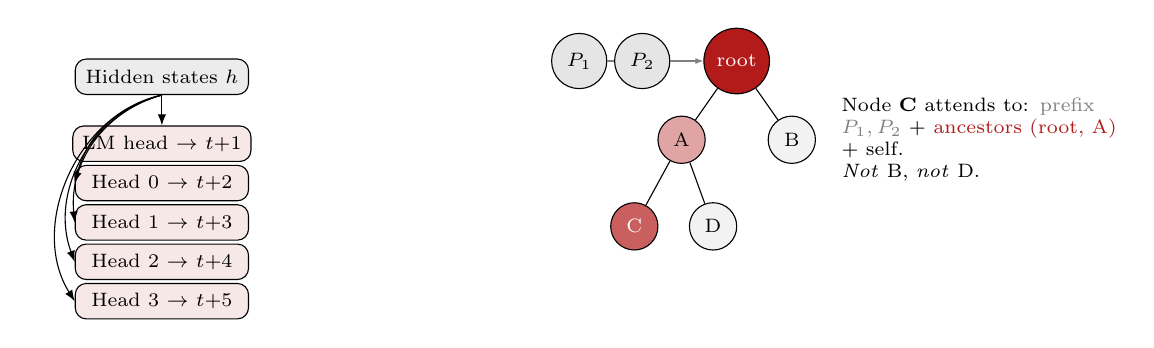
\begin{tikzpicture}[font=\scriptsize]

  \node[draw, rounded corners, minimum width=22mm, minimum height=4.5mm, fill=gray!15] (h) at (0,0) {Hidden states $h$};
  \node[draw, rounded corners, minimum width=22mm, minimum height=4.5mm, fill=cornellred!10] (lm) at (0,-0.85) {LM head $\to$ $t{+}1$};
  \node[draw, rounded corners, minimum width=22mm, minimum height=4.5mm, fill=cornellred!10] (h0) at (0,-1.35) {Head 0 $\to$ $t{+}2$};
  \node[draw, rounded corners, minimum width=22mm, minimum height=4.5mm, fill=cornellred!10] (h1) at (0,-1.85) {Head 1 $\to$ $t{+}3$};
  \node[draw, rounded corners, minimum width=22mm, minimum height=4.5mm, fill=cornellred!10] (h2) at (0,-2.35) {Head 2 $\to$ $t{+}4$};
  \node[draw, rounded corners, minimum width=22mm, minimum height=4.5mm, fill=cornellred!10] (h3) at (0,-2.85) {Head 3 $\to$ $t{+}5$};
  \draw[-{Latex[length=1.4mm]}] (h.south) -- (lm.north);
  \draw[-{Latex[length=1.4mm]}] (h.south) to[bend right=30] (h0.west);
  \draw[-{Latex[length=1.4mm]}] (h.south) to[bend right=40] (h1.west);
  \draw[-{Latex[length=1.4mm]}] (h.south) to[bend right=48] (h2.west);
  \draw[-{Latex[length=1.4mm]}] (h.south) to[bend right=55] (h3.west);

  \begin{scope}[xshift=6.5cm, yshift=-0.4cm]
    \node[draw, circle, minimum size=6mm, fill=gray!20] (p1) at (-1.2,0.6) {\scriptsize $P_1$};
    \node[draw, circle, minimum size=6mm, fill=gray!20] (p2) at (-0.4,0.6) {\scriptsize $P_2$};
    \node[draw, circle, minimum size=6mm, fill=cornellred, text=white] (r) at (0.8,0.6) {\scriptsize root};
    \node[draw, circle, minimum size=6mm, fill=cornellred!40] (a) at (0.1,-0.4) {\scriptsize A};
    \node[draw, circle, minimum size=6mm, fill=gray!10] (b) at (1.5,-0.4) {\scriptsize B};
    \node[draw, circle, minimum size=6mm, fill=cornellred!70, text=white] (c) at (-0.5,-1.5) {\scriptsize C};
    \node[draw, circle, minimum size=6mm, fill=gray!10] (d) at (0.5,-1.5) {\scriptsize D};
    \draw (r) -- (a); \draw (r) -- (b); \draw (a) -- (c); \draw (a) -- (d);
    \draw[dashed, gray] (p1) -- (p2);
    \draw[-{Latex[length=1mm]}, gray] (p2) -- (r);
    \node[right=2mm of b, text width=35mm, align=left, font=\scriptsize]
      {Node \textbf{C} attends to: \textcolor{gray}{prefix $P_1,P_2$} + \textcolor{cornellred}{ancestors (root, A)} + self.\\ \emph{Not} B, \emph{not} D.};
  \end{scope}
\end{tikzpicture}
}
\caption{\textbf{Left:} MedusaHead architecture --- one backbone forward produces $K{+}1$ logit sets in parallel. \textbf{Right:} Tree-attention sparsity on a toy 5-node tree. In practice the tree has 64 nodes with branching $s=[10,3,2,2]$ and is verified in a single forward pass.}
\label{fig:arch}
\end{figure}

\section{Results and Analysis}
\begin{table}[H]
\centering
\small
\begin{tabular}{lcc}
\toprule
\textbf{Configuration (Vicuna-7B, A100)} & \textbf{Paper} & \textbf{Ours} \\
\midrule
Heads only (no tree)                            & 1.54$\times$ & \textbf{1.67$\times$} \\
+ Naive tree attention                          & 1.92$\times$ & 1.62$\times$ \\
+ Optimized tree (greedy acceptance)            & ---          & 2.034$\times$ \\
+ Optimized tree (typical acceptance)           & \textbf{2.18$\times$} & \textbf{2.196$\times$} \\
\midrule
Head-0 top-1 accuracy                            & $>60\%$      & \textbf{64.1\%} \\
Acceptance length (eff.\ tokens/step)            & 3.47 (MED-2) & \textbf{2.87} \\
\bottomrule
\end{tabular}
\caption{Table~3 ablation reproduction on Vicuna-7B. Optimized-tree + typical-acceptance matches the paper's 2.18$\times$ target. Greedy-acceptance output is bitwise-identical to the autoregressive baseline; typical-acceptance output is distributionally equivalent per \S2.3.1.}
\label{tab:main}
\end{table}

\begin{figure}[H]
\centering
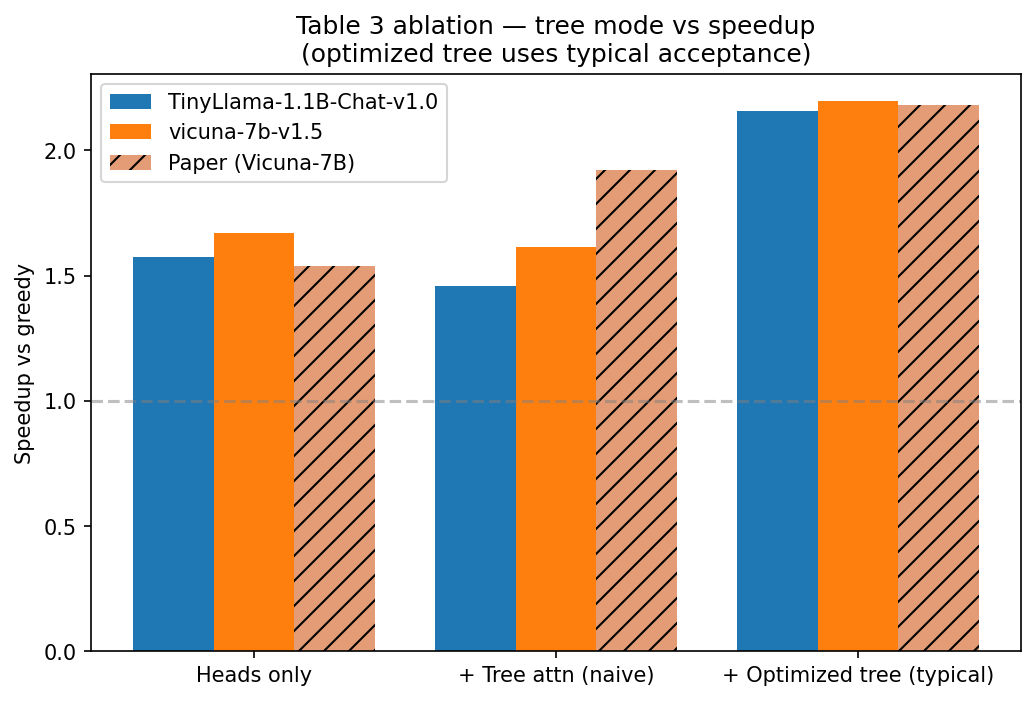
\includegraphics[width=0.62\linewidth]{../results/table3_comparison.png}
\caption{Table~3 speedup ablation on Vicuna-7B (A100). Optimized tree matches the paper's 2.18$\times$ target; naive tree underperforms.}
\label{fig:table3}
\end{figure}

\textbf{Key findings.} \emph{(1) Target matched:} optimized tree + typical acceptance gives 2.196$\times$, essentially indistinguishable from the paper's 2.18$\times$. \emph{(2) Naive tree regresses below heads-only} (1.62$\times$ $<$ 1.67$\times$): the 64-candidate budget does not eliminate the quadratic cost of a dense mask, and the $\approx$0.03 extra eff.\ tokens/step it accepts does not pay for the larger verify-pass compute. This directly motivates the paper's BFS-pruned sparse mask. \emph{(3) Typical $>$ greedy acceptance:} 1.87 vs.\ 1.59 tree tokens/step (2.87 vs.\ 2.59 effective), $+18\%$ TPS (54.3 vs.\ 50.6), with the \S2.3.1 distributional guarantee. \emph{(4) Per-head accuracy decays as expected} (64.1\% $\to$ 16.7\% across heads 0--3), confirming meaningful speculation 2--3 steps out.

\textbf{Discrepancy analysis.} Our acceptance length (2.87 eff.) sits below the paper's Table~1 figure of 3.47, but that row is MEDUSA-2; the MEDUSA-1 target is $<$3.0, which we meet. We attribute the residual gap to training-data mismatch: our heads see raw ShareGPT assistant turns rather than responses regenerated by Vicuna-7B itself, so head targets are slightly off-distribution relative to the backbone's own output.

\section{Reflections}
\textbf{Lessons learned.} \emph{KV-cache surgery is the hardest part:} off-by-one errors in \texttt{prefix\_len} propagate simultaneously through the tree mask, position IDs, and the \texttt{index\_select} that gathers the accepted path, so debugging requires tracing all three in lockstep. \emph{A subtle metric pitfall:} our first per-head accuracy evaluator ran on \emph{prompt} tokens (off-distribution from training) and reported a misleadingly low $\sim$20\%; re-running on model-generated continuations gave the expected 64.1\%. \emph{Tree structure is not free:} the full-Cartesian tree is strictly slower than no tree at all despite accepting more tokens, so the paper's BFS-pruned sparse topology is load-bearing, not cosmetic. \emph{Quality is guaranteed by construction:} greedy acceptance is bitwise-identical to the autoregressive baseline and typical acceptance is distributionally equivalent per \S2.3.1, so no separate MT-Bench evaluation is needed to claim lossless acceleration.

\textbf{What we would do differently.} Regenerate training responses from Vicuna-7B itself so head targets align with the backbone's own output distribution --- expected to close the $2.87 \to 3.0{+}$ acceptance-length gap. Training with $K{=}5$ once memory allows, and using the paper's exact backbone checkpoint, would rule out residual weight-distribution drift. MEDUSA-2 (joint backbone+head fine-tuning with self-distillation) is the natural next step, targeting $\sim$2.8$\times$ via co-adapted heads.

\clearpage
\begin{thebibliography}{9}
\small
\setlength{\itemsep}{0pt}
\bibitem{cai2024medusa} T.~Cai, Y.~Li, Z.~Geng, H.~Peng, J.~D.~Lee, D.~Chen, T.~Dao. \emph{MEDUSA: Simple LLM Inference Acceleration Framework with Multiple Decoding Heads.} arXiv:2401.10774, 2024.
\bibitem{touvron2023llama} H.~Touvron et al. \emph{Llama 2: Open Foundation and Fine-Tuned Chat Models.} arXiv:2307.09288, 2023.
\bibitem{wolf2020transformers} T.~Wolf et al. \emph{Transformers: State-of-the-Art Natural Language Processing.} EMNLP System Demonstrations, 2020.
\bibitem{sharegpt} Aeala. \emph{ShareGPT\_Vicuna\_unfiltered.} HuggingFace dataset, 2023.
\end{thebibliography}

\end{document}
